\documentclass[../design_fonctionnement_sys.tex]{subfiles}
\begin{document}

\section{Fonctionnement du système}
Cette section portera sur des diagrammes qui présenteront le fonctionnement de différentes parties du système.

\subsection{Inscription}
Si le joueur possède déjà un compte, il a la possibilité de se connecter directement.
Le gestionnaire d'inscription (registerController) effectuera une première vérification des données saisies par l'utilisateur, 
notamment en s'assurant qu'aucun champ n'est laissé vide. 
Une fois cette vérification effectuée, les données seront transmises au serveur. 
Ce dernier procédera ensuite à la vérification de la disponibilité du nom d'utilisateur.

\begin{figure}[H]
    \centering
    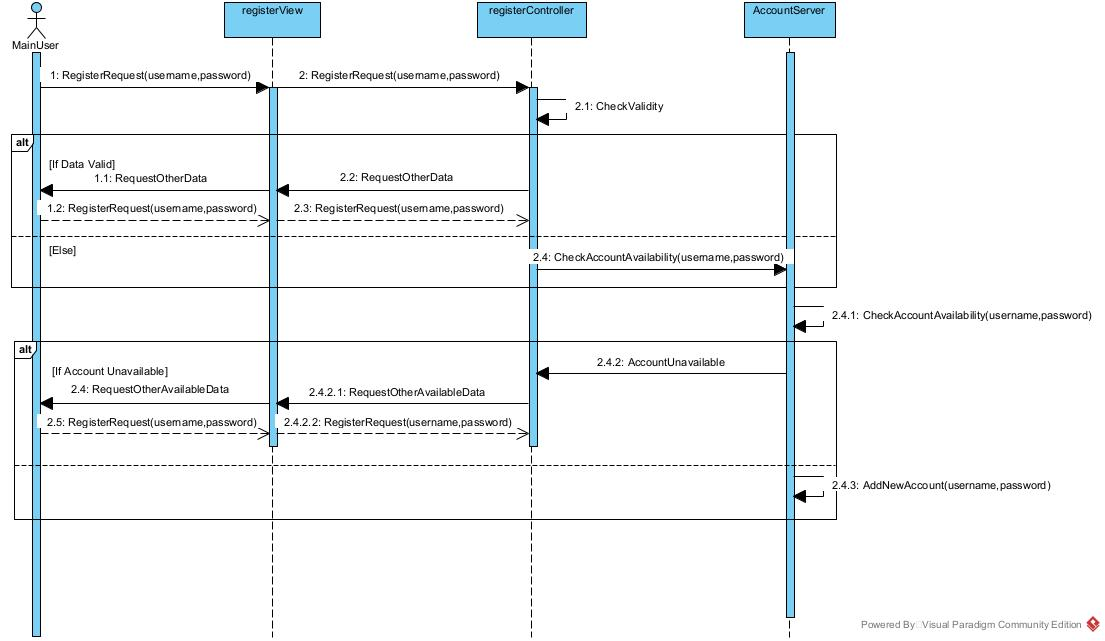
\includegraphics[scale=0.4]{img_design/RegisterSD.jpg}
    \label{fig:seq_match_client}
    \caption{Inscription}
\end{figure}
\newpage

\subsection{Connexion}
Afin d'assurer la connexion et l'inscription des joueurs, une classe \texttt{AccountServer} qui assure la communication avec la base de donnée. 
Quand un joueur demande de se connecter, la méthode de \texttt{checkAccount} 
de la classe permet de vérifier qu'un joueur a entré le bon mot de passe, si oui, 
une instance de classe \texttt{ConnectedUser} est crée avec le socket du joueur et les informations de comptes du joueur. 
Une réponse est envoyée qui précise si le joueur est connecté, ou, dans le cas contraitre, s'il a rentré des informations non valides.
\begin{figure}[H]
    \centering
    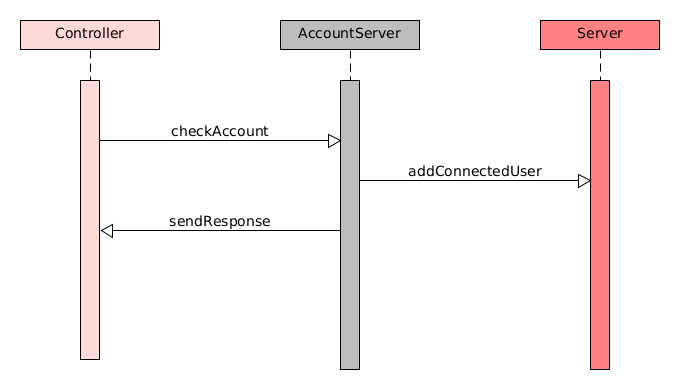
\includegraphics[scale=0.4]{img_design/connexion_seq.png}
    \label{fig:seq_match_client}
    \caption{Connexion}
\end{figure}


\subsection{Chat}
Un utilisateur a le choix d'envoyer un message à un ou plusieurs utilisateurs, le message est récupéré et transmis
au(x) utilisateur(s) par le ChatServer, et afficher par l'intermédiaire de ChatView.
\begin{figure}[H]
    \centering
    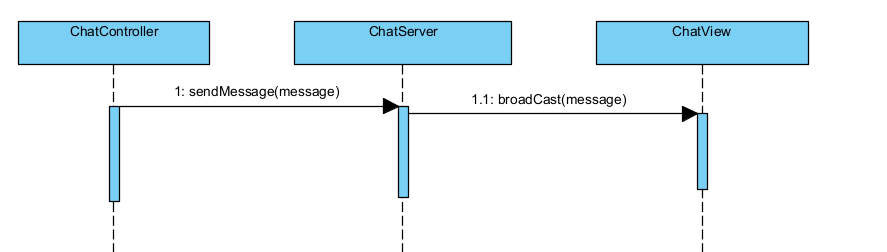
\includegraphics[scale=0.3]{img_design/Chat_DS.png}
    \label{fig:seq_match_client}
    \caption{Envoie d'un message}
\end{figure}

\newpage

\subsection{Matchmaking}
Ce diagramme décrit la séquence d'actions réalisés lorsqu'un utilisateur veut créer/configurer une partie.

\begin{figure}[H]
    \centering
    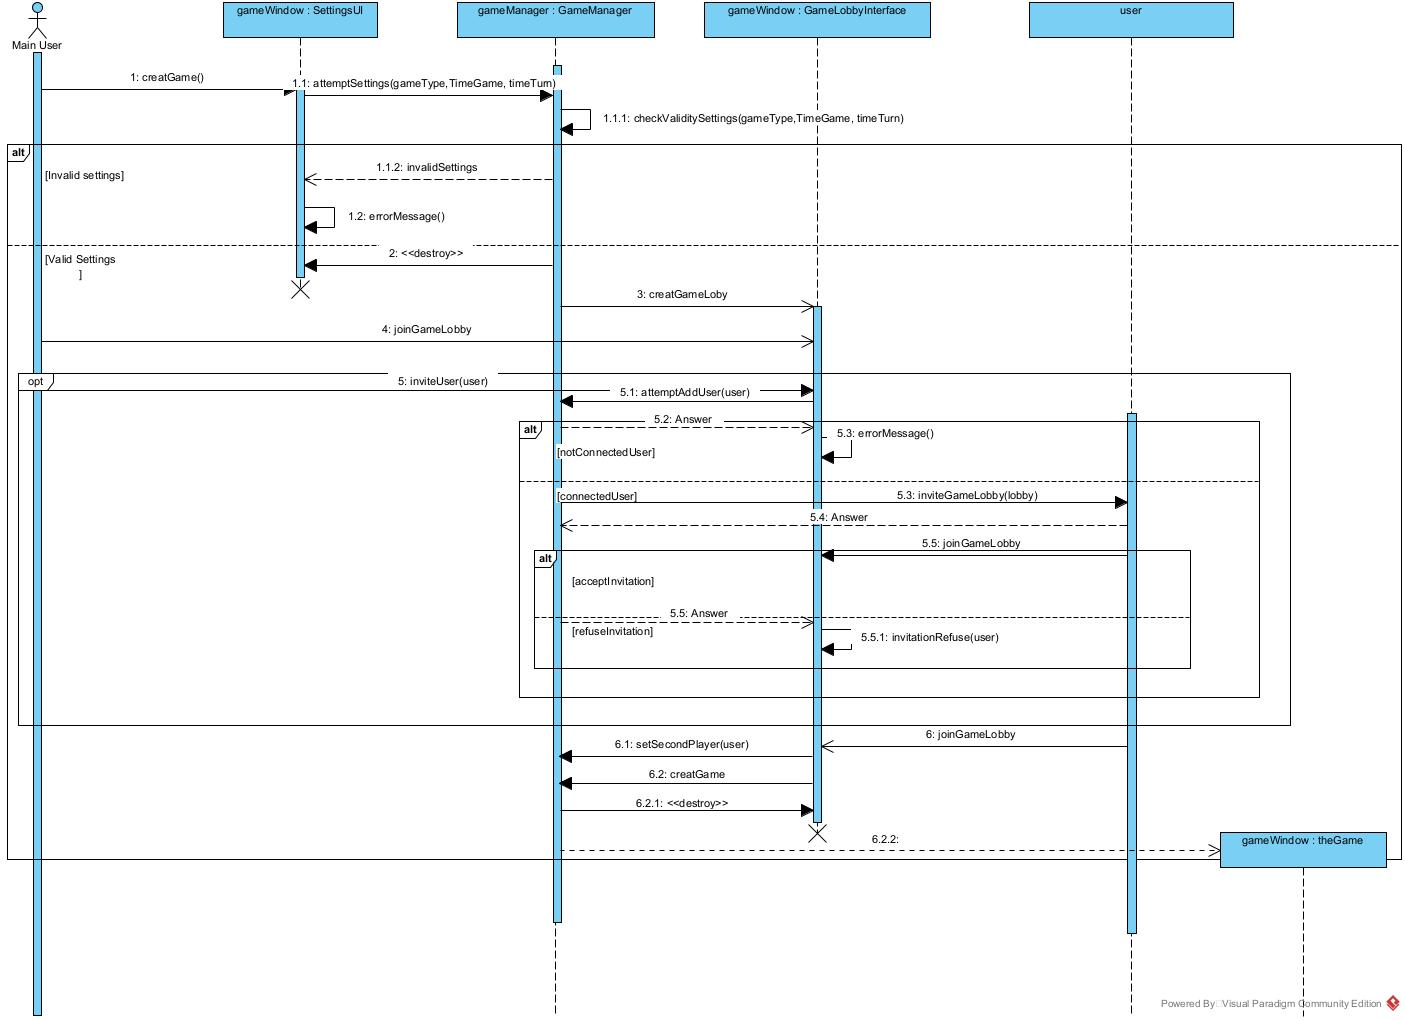
\includegraphics[scale=0.3]{img_design/PreLoby.jpg}
    \label{fig:seq_match_client}
    \caption{Matchmaking : Création du lobby}
\end{figure}

\newpage

\subsection{Lobby}
Ce diagramme décrit la séquence d'actions réalisés lorsqu'un utilisateur se trouve au stade de lobby et qu'il veut démarrer une partie.
Le deuxième joueur a déjà été fixé, et les bateaux doivent être placés sur le plateau pour que la partie puisse se lancer.
Mais avant de placer les bateaux, le plateau avec les deux boards est créé mais aussi 2 players. Un player est assigné à chaque user.

\begin{figure}[H]
    \centering
    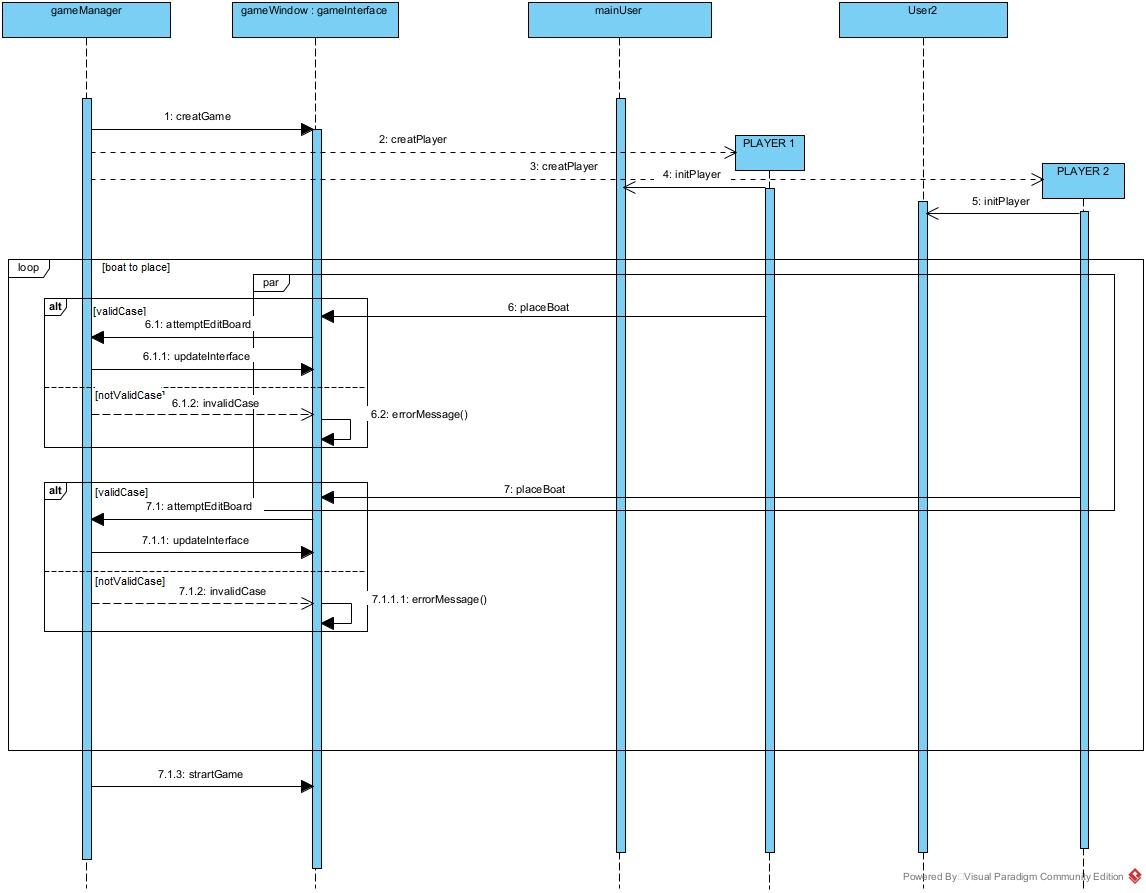
\includegraphics[scale=0.4]{img_design/PreGame.jpg}
    \label{fig:seq_match_server}
    \caption{Avant que la partie commence}
\end{figure}
\newpage

\subsection{Boucle de jeu}
La déroulement de la partie se passe au tour par tour. A tour de rôle le user transmet son action
mais l'action est gérée par player. Cela permet à une classe player d'avoir des points d'énergie, des actions et faire partie
d'une faction. L'action est d'abbord vérifiée pour savoir si la case ciblée est autorisée. Si c'est le cas le plateau
est modifié et l'interface est mise à jour.

\begin{figure}[H]
    \centering
    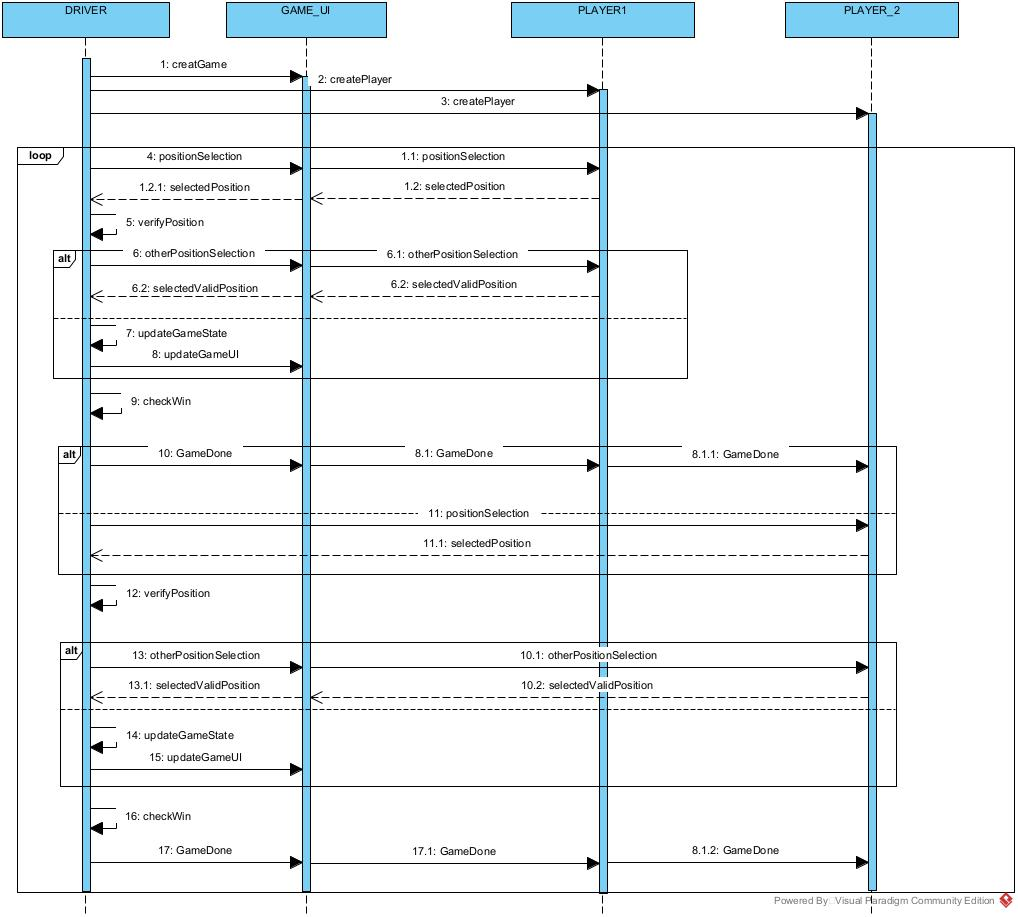
\includegraphics[scale=0.3]{img_design/Game.jpg}
    \label{fig:seq_gameloop_client}
    \caption{Boucle de jeu}
\end{figure}



\end{document}